%% LyX 2.1.2 created this file.  For more info, see http://www.lyx.org/.
%% Do not edit unless you really know what you are doing.
\documentclass[english,aps,reprint]{revtex4-1}
\usepackage[T1]{fontenc}
\usepackage[latin9]{inputenc}
\setcounter{secnumdepth}{3}
\usepackage{bm}
\usepackage{amsmath}
\usepackage{graphicx}

\makeatletter
%%%%%%%%%%%%%%%%%%%%%%%%%%%%%% Textclass specific LaTeX commands.
% Fix a couple of bugs in REVTeX 4.1
\def\lovname{List of Videos}
\@ifundefined{textcolor}{}
{%
 \definecolor{BLACK}{gray}{0}
 \definecolor{WHITE}{gray}{1}
 \definecolor{RED}{rgb}{1,0,0}
 \definecolor{GREEN}{rgb}{0,1,0}
 \definecolor{BLUE}{rgb}{0,0,1}
 \definecolor{CYAN}{cmyk}{1,0,0,0}
 \definecolor{MAGENTA}{cmyk}{0,1,0,0}
 \definecolor{YELLOW}{cmyk}{0,0,1,0}
}

%%%%%%%%%%%%%%%%%%%%%%%%%%%%%% User specified LaTeX commands.
\usepackage{fullpage}

\makeatother

\usepackage{babel}
\begin{document}

\title{Hydrodynamic Synchronization of optically trapped micro-beads}

\maketitle

\section{introduction}

Hydrodynamic interaction plays an important role in the dynamics of microscopic particles.
In a simple experimental setup using two optical traps, trapping a microbead each,
we study the response of the second bead when first bead is driven with periodic
force. We have further developed a theory to study and analyzed the experimental
results. 

The force balance equation of the optically trapped bead is,\begin{subequations}\

\begin{alignat}{1}
m\dot{\mathbf{v}}_{i} & =-\bm{\gamma}_{ij}\mathbf{v}_{j}-\bm{\nabla}_{i}U+\bm{\xi}_{i}\\
\dot{\mathbf{R}}_{i} & =\mathbf{v}_{i}
\end{alignat}
\end{subequations}

In the above Eq. $\mathbf{R}_{i}$ and $\mathbf{v}_{i}$ are position and velocity
of the $i$-th particle of mass $m$, $\bm{\gamma}_{ij}$ is manybody friction tensor
and $U$ is the potential and $\xi$ is noise of thermal origin. In a optical trap,
the potential is \textbf{$U(t)=\frac{1}{2}\sum k_{i}(\mathbf{R}_{i}-\mathbf{R}_{i}^{0})^{2}$}
with $\mathbf{R}_{i}^{0}$ is the position of the potential minimum of the $i$-th
optical trap. In the experimental set up the minimum of the optical trap is shifting
with a periodic signal from outside and the response of the two beads have been studied.
Assuming momentum to be rapidly relaxing on the time scale of the trap motion, we
neglect inertia and average over the noise to get,
\begin{alignat}{1}
-\bm{\gamma}_{ij}\mathbf{\dot{R}}_{j} & -\bm{\nabla}_{i}U=0\label{eq:fric}
\end{alignat}
Eq.(2) can be inverted and presented in terms of mobility matrices as,
\begin{eqnarray}
\negthickspace\negthickspace\mathbf{\dot{R}}_{1} & = & -\mu\bm{\delta}k_{1}(\mathbf{R}_{1}-\mathbf{R}_{1}^{0})-\bm{\mu}_{12}k_{2}(\mathbf{R}_{2}-\mathbf{R}_{2}^{0})\nonumber \\
\negthickspace\negthickspace\mathbf{\dot{R}}_{2} & = & -\bm{\mu}_{21}k_{1}(\mathbf{R}_{1}-\mathbf{R}_{1}^{0})-\mu\bm{\delta}k_{2}(\mathbf{R}_{2}-\mathbf{R}_{2}^{0})
\end{eqnarray}


Approximate mobility matrices with separation vector to be the average distance between
two minimum of the optical traps. Thus we get,
\begin{eqnarray}
\negthickspace\frac{d}{dt}\left[\begin{array}{c}
\mathbf{R}_{1}\\
\mathbf{R}_{2}
\end{array}\right] & = & -\left[\begin{array}{cc}
\mu k_{1}\bm{\delta} & \bm{\mu}_{12}k_{2}\\
\bm{\mu}_{21}k_{1} & \mu k_{2}\bm{\delta}
\end{array}\right]\negthickspace\left[\begin{array}{c}
\mathbf{R}_{1}\\
\mathbf{R}_{2}
\end{array}\right]\nonumber \\
 &  & +\left[\begin{array}{cc}
\mu\bm{\delta} & \bm{\mu}_{12}\\
\bm{\mu}_{21} & \mu\bm{\delta}
\end{array}\right]\negthickspace\left[\begin{array}{c}
\mathbf{F}_{1}^{0}\\
\mathbf{F}_{2}^{0}
\end{array}\right]
\end{eqnarray}


Steady state solution of the Eq.(4) can easily be calculated by taking Fourier transformation.
Assuming $\mathbf{A}=\left[\begin{array}{cc}
\mu k_{1}\bm{\delta} & \bm{\mu}_{12}k_{2}\\
\bm{\mu}_{21}k_{1} & \mu k_{2}\bm{\delta}
\end{array}\right]$ and $\mathbf{M}=\left[\begin{array}{cc}
\mu\bm{\delta} & \bm{\mu}_{12}\\
\bm{\mu}_{21} & \mu\bm{\delta}
\end{array}\right]$, the solution in frequency is
\begin{equation}
\mathbf{R}_{i}(\omega)=[-i\omega\bm{\delta}+\mathbf{A}]_{ij}^{-1}\mathbf{M}\mathbf{F}_{j}^{0}(\omega)=\bm{\chi}_{ij}(\omega)\mathbf{F}_{j}^{0}(\omega)
\end{equation}
which defines the response for $\bm{\chi}$. 

As the minimum of the optical trap is modulated by a sinusoidal wave with driving
frequency $\Omega$, $\mathbf{F}_{j}^{0}(\omega)=\frac{\mathbf{X}_{j}}{2}(\delta(\omega-\Omega)+\delta(\omega+\Omega)).$
Further $\bm{\chi}$ is a block-diagonal matrix in cartesian indices. Given the experimental
set up $\bm{\chi}$ can be decomposed in $\bm{\chi}_{\parallel}$and $\bm{\chi}_{\perp}$for
motion along the trap separation and the motion perpendicular to it. Inserting this
form of the signal into the Eq. above and taking the response equation back to time
domain, we find

\begin{equation}
\negthickspace R_{\parallel i}(t)=\chi_{\parallel ij}'(\Omega)\cos(\Omega t)X_{j}+\chi_{\parallel ij}''(\Omega)\sin(\Omega t)X_{j}
\end{equation}
Two time scales from two traps can be calculated to be $\tau_{i}=1/\mu k_{i}$. 
\begin{figure*}
\includegraphics[width=1.05\textwidth]{chi11}

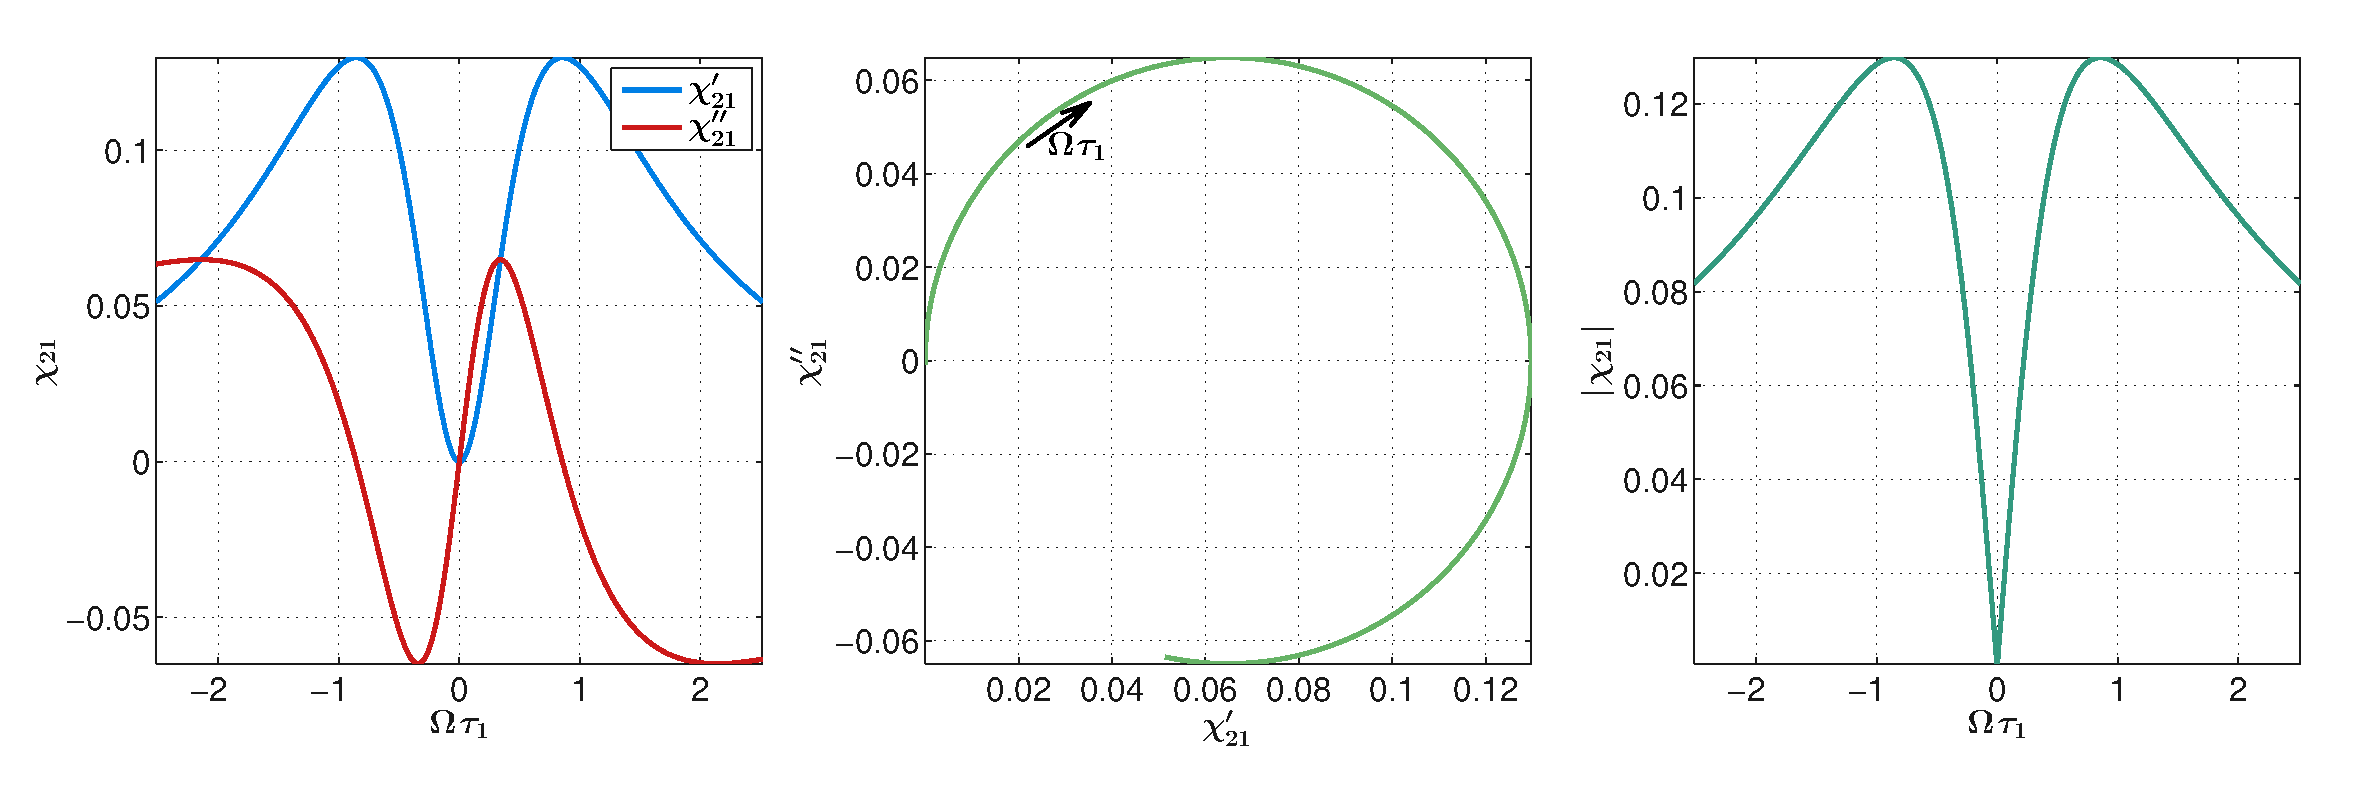
\includegraphics[width=1.05\textwidth]{chi21}

\protect\caption{Real and imaginary part of the response function(a). Cole-Cole plot (b) and the amplitude
of the response function.}
\end{figure*}
\begin{widetext}

\begin{alignat}{1}
\bm{\chi}_{\parallel}(\Omega) & =\left[\begin{array}{cc}
(\mu k_{1}-i\Omega) & \mu_{12}k_{2}\\
\\
\mu_{21}k_{1} & (\mu k_{2}-i\Omega)
\end{array}\right]^{-1}\left[\begin{array}{cc}
\mu & \mu_{12}\\
\mu_{21} & \mu
\end{array}\right]\nonumber \\
 & =\frac{1}{Det\, A_{\parallel}-\Omega^{2}-i\Omega Tr\, A_{\parallel}}\left[\begin{array}{cc}
(\mu k_{2}-i\Omega) & -\mu_{12}k_{2}\\
\, & \,\\
-\mu_{21}k_{1} & (\mu k_{1}-i\Omega)
\end{array}\right]\left[\begin{array}{cc}
\mu & \mu_{12}\\
\mu_{21} & \mu
\end{array}\right]\nonumber \\
 & =\frac{Det\, A_{\parallel}-\Omega^{2}+i\Omega Tr\, A_{\parallel}}{(Det\, A_{\parallel}-\Omega^{2})^{2}+\Omega^{2}(Tr\, A_{\parallel})^{2}}\left[\begin{array}{cc}
k_{2}DetM_{\parallel}-i\mu\Omega & -i\Omega\mu_{12}\\
\, & \,\\
-i\Omega\mu_{21} & k_{1}DetM_{\parallel}-i\mu\Omega
\end{array}\right]\nonumber \\
\bm{\chi}_{\parallel}^{'}(\Omega) & =\frac{1}{(Det\, A_{\parallel}-\Omega^{2})^{2}+\Omega^{2}(Tr\, A_{\parallel})^{2}}\left[\begin{array}{cc}
\begin{array}{c}
k_{2}DetA_{\parallel}DetM_{\parallel}\\
+\Omega^{2}(k_{2}\mu_{12}\mu_{21}+k_{1}\mu^{2})
\end{array} & \Omega^{2}Tr\, A_{\parallel}\mu_{12}\\
{\displaystyle \Omega^{2}Tr\, A_{\parallel}\mu_{12}} & \begin{array}{c}
k_{1}DetA_{\parallel}DetM_{\parallel}\\
+\Omega^{2}(k_{1}\mu_{12}\mu_{21}+k_{2}\mu^{2})
\end{array}
\end{array}\right]\nonumber \\
\nonumber \\
\bm{\chi}_{\parallel}^{''}(\Omega) & =\frac{\Omega}{(Det\, A_{\parallel}-\Omega^{2})^{2}+\Omega^{2}(Tr\, A_{\parallel})^{2}}\left[\begin{array}{cc}
{\displaystyle \mu k_{2}^{2}DetM_{\parallel}+\mu\Omega^{2}} & -(Det\, A_{\parallel}-\Omega^{2})\mu_{12}\\
\\
-(Det\, A_{\parallel}-\Omega^{2})\mu_{21} & \mu k_{1}^{2}DetM_{\parallel}+\mu\Omega^{2}
\end{array}\right]\label{eq:ImRes2}
\end{alignat}
\end{widetext}

We are interested in the resonance in amplitude of the second bead due to the forcing
of the first bead, that is given by the maximising modulus of $\chi_{\parallel21}$
with respect to $\Omega$. 
\begin{eqnarray*}
|\chi_{21}| & =\big| & \frac{-i\Omega\mu_{21}}{Det\, A_{\parallel}-\Omega^{2}-i\Omega Tr\, A_{\parallel}}\big|\\
 & = & \frac{\Omega\mu_{21}}{\sqrt{\left(Det\, A_{\parallel}-\Omega^{2}\right)^{2}+\Omega^{2}(Tr\, A_{\parallel})^{2}}}
\end{eqnarray*}


Clearly the resonance frequency in dimensionless unit is $\tau_{1}\Omega_{res}=\sqrt{\frac{DetA_{\parallel}}{\mu^{2}k_{1}^{2}}}=\sqrt{\frac{k_{2}}{k_{1}}\left(1-\frac{\mu_{\parallel12}^{2}}{\mu^{2}}\right)}$
when $\mu_{21}\neq0$.

Now lets consider there is no external force but two particles are moving in the
trap because of thermal fluctuation. Then from Eq.\ref{eq:fric} we can get
\begin{gather*}
\gamma_{ij}\dot{R}_{j}=-k_{ij}R_{j}+\xi_{i}\\
\langle\xi_{j}\rangle=0\\
\langle\xi_{i}\xi_{j}\rangle=2k_{B}T\gamma_{ij}
\end{gather*}
Steady state solution in frequency space can be derived easily by Fourier transform
\[
\mathbf{R}(\omega)=(-i\omega\bm{\delta}+\mathbf{A})^{-1}\mathbf{M}\bm{\xi}(\omega)
\]
Correlation matrix become
\begin{eqnarray}
\langle\mathbf{R}(\omega)\mathbf{R}^{\dagger}(\omega)\rangle & = & (-i\omega\bm{\delta}+\mathbf{A})^{-1}\mathbf{M}\langle\bm{\xi}(\omega)\bm{\xi}^{\dagger}(\omega)\rangle\mathbf{M}(i\omega\bm{\delta}+\mathbf{A}^{T})^{-1}\nonumber \\
\frac{1}{2k_{B}T}\, C_{\Delta\Delta} & = & (-i\omega\bm{\delta}+\mathbf{A})^{-1}\mathbf{M}(i\omega\bm{\delta}+\mathbf{A}^{T})^{-1}\label{eq:Corr2}
\end{eqnarray}
\begin{widetext}

\[
(-i\omega\bm{\delta}+\mathbf{A}_{\parallel})^{-1}\mathbf{M}_{\parallel}(i\omega\bm{\delta}+\mathbf{A}_{\parallel}^{T})^{-1}=\frac{1}{(Det\, A_{\parallel}-\omega^{2})^{2}+\omega^{2}(Tr\, A_{\parallel})^{2}}\left[\begin{array}{cc}
\mu k_{2}-i\omega & -\mu_{12}k_{2}\\
-\mu_{21}k_{1} & \mu k_{1}-i\omega
\end{array}\right]\left[\begin{array}{cc}
\mu & \mu_{12}\\
\mu_{21} & \mu
\end{array}\right]\left[\begin{array}{cc}
\mu k_{2}+i\omega & -\mu_{21}k_{1}\\
-\mu_{12}k_{2} & \mu k_{1}+i\omega
\end{array}\right]
\]


\begin{align}
 & \left[\begin{array}{cc}
\mu k_{2}-i\omega & -\mu_{12}k_{2}\\
\, & \,\\
-\mu_{21}k_{1} & \mu k_{1}-i\omega
\end{array}\right]\left[\begin{array}{cc}
\mu & \mu_{12}\\
\, & \,\\
\mu_{21} & \mu
\end{array}\right]\left[\begin{array}{cc}
\mu k_{2}+i\omega & -\mu_{21}k_{1}\\
\, & \,\\
-\mu_{12}k_{2} & \mu k_{1}+i\omega
\end{array}\right]\nonumber \\
= & \left[\begin{array}{cc}
k_{2}DetM_{\parallel}-i\omega\mu & -i\omega\mu_{12}\\
\, & \,\\
-i\omega\mu_{21} & k_{1}DetM_{\parallel}-i\omega\mu
\end{array}\right]\left[\begin{array}{cc}
\mu k_{2}+i\omega & -\mu_{21}k_{1}\\
\, & \,\\
-\mu_{12}k_{2} & \mu k_{1}+i\omega
\end{array}\right]\nonumber \\
= & \left[\begin{array}{cc}
(k_{2}DetM_{\parallel}-i\omega\mu)(\mu k_{2}+i\omega)+i\omega\mu_{12}^{2}k_{2} & -(k_{2}DetM_{\parallel}-i\omega\mu)\mu_{21}k_{1}-(\mu k_{1}+i\omega)i\omega\mu_{12}\\
\, & \,\\
-(k_{1}DetM_{\parallel}-i\omega\mu)\mu_{12}k_{2}-(\mu k_{2}+i\omega)i\omega\mu_{21} & (k_{1}DetM_{\parallel}-i\omega\mu)(\mu k_{1}+i\omega)+i\omega\mu_{21}^{2}k_{1}
\end{array}\right]\nonumber \\
= & \left[\begin{array}{cc}
\mu k_{2}^{2}DetM_{\parallel}+\mu\omega^{2} & -(DetA_{\parallel}-\omega^{2})\mu_{21}\\
\, & \,\\
-(DetA_{\parallel}-\omega^{2})\mu_{12} & \mu k_{1}^{2}DetM_{\parallel}+\mu\omega^{2}
\end{array}\right]\label{eq:CorrMatmul}
\end{align}


\end{widetext}

Now reading off the equations \ref{eq:ImRes2}, \ref{eq:Corr2}, \ref{eq:CorrMatmul},
we can easily see that Fluctuation-dissipation holds. It comes out to be in matrix
form as,
\[
2k_{B}T\times Im\left\{ \bm{\chi}''(\omega)\right\} =\omega\mathbf{C}_{xx}(\omega)
\]


\appendix

\section{One independent harmonic oscillator}

For the case of a one dimensional harmonic oscillator, the equation can be written
as
\begin{eqnarray}
m\dot{v} & = & -\gamma v-k(x-x^{0})+\xi\\
\dot{x} & = & v
\end{eqnarray}


Clearly, for over-damed limit of the equation, we can neglect the mass term and force
balance equation can be written as,
\begin{eqnarray}
\gamma v & = & -kx+kx^{0}+\xi
\end{eqnarray}
where distribution for noise follow $\langle\xi\rangle=0$,$\langle\xi\xi\rangle=2k_{B}T\gamma$.
Inverting the equation we get,
\begin{eqnarray*}
\dot{x} & = & -\mu kx+\mu kx^{0}+\mu\xi
\end{eqnarray*}
 The steady state solution for average in frequency space is
\begin{alignat}{1}
x(\omega) & =\frac{{\displaystyle \mu kx^{0}(\omega)}}{{\displaystyle (-i\omega+\mu k)}}=\chi(\omega)f(\omega)\\
\chi(\omega) & =\frac{(\mu k+i\omega)\mu}{\omega^{2}+\mu^{2}k^{2}}\nonumber \\
\chi''(\omega) & =\frac{\mu\omega}{\omega^{2}+\mu^{2}k^{2}}\label{eq:img}
\end{alignat}
If there is no external force we can calculate the auto-correlation function
\begin{alignat}{1}
C_{xx}(\omega) & =\langle x(\omega)x^{\ast}(\omega)\rangle\\
 & =\langle\frac{\mu\xi(\omega)}{(-i\omega+\mu k)}\frac{\xi^{\ast}(\omega)\mu}{(i\omega+\mu k)}\rangle\nonumber \\
 & =\frac{2k_{B}T\mu\gamma\mu}{\omega^{2}+\mu^{2}k^{2}}=\frac{2k_{B}T\mu}{\omega^{2}+\mu^{2}k^{2}}\label{eq:cor}
\end{alignat}
Generalised form of fluctuation dissipation theorem connects correlation to the imaginary
part of the response function as
\begin{equation}
2k_{B}T\chi''(\omega)=\omega C_{xx}(\omega)
\end{equation}


We can read of imaginary part of the response and correlation function directly from
Eq.\ref{eq:img} and Eq.\ref{eq:cor} respectively and confirm fluctuation dissipation
theorem in one dimentional harmonic oscillator context. 
\end{document}
